\chapter{State of the Art: Literature Review and Recent Developments}\label{Chap2}
\echapter{State of the Art: Literature Review and Recent Developments}

\section{Highlights}\label{Chap2_01}
\esection{Highlights}
\begin{itemize}
\item 1. Theoretical tools initiated by many researchers:
Solder voids
IMC growth under electric field

\item 2. Utilization of Synchrotron Radiation Experimental Set Up.

\item 3. Numerical Methods and Computational Softwares

\item 4. CALPHAD and Chemical Kinetics Analysis 
\end{itemize}

\section{Introduction}\label{Chap2_01}
\esection{Introduction}
In order to consolidate the aspects related to the study of interfacial bubbles and intermetallic compounds in solder joints, it is a good idea to highlight the (i) ongoing research approaches by the investigators,(ii) introductory background of novel experimental method utilized in this study, (iii) object-oriented concepts on CALPHAD and chemical kinetics as well as (iv) brief presentation of the relevant numerical methods and computational softwares. This chapter is thus focused on these materials. Section 2.2 is concerned with the outlining of research activities performed by several scientists and engineers in the fields of voids and field-gradient related IMC. This  is followed by the explanation of the synchrotron radiation imaging technique and its potential benefits in the microstructural analysis in solder joints (section 2.3). The concepts on CALPHAD and chemical kinetics associated with present study are outlined in section 2.4. The last portion of this chapter i.e. section 2.5 is devoted to the description of the numerical methods namely- finite element  and finite volume methods. Also,in this section, several computer based softwares such as Elmer, FiPy, MOOSE, OpenCalphad and Cantera are described.
\section{Research Trends about Interfacial Voids in Lead-free Solders}
\esection{Research Trends about Interfacial Voids in Lead-free Solders}
\paragraph*{•}
The cause for formation and growth factors of voids in solder - Cu$_6$Sn$_5$ interface during multireflow soldering has been investigated by Lin and Luo ~\cite{XLin2007}. It has been found in the study that the volume shrinkage during the phase transformation leads to appearance of the voids.The growth rate of the void has been connected with the initial morphology of the IMC. The maximum sizes of these voids has been described to be around 3 $\mu$m. Sangil Lee and coworkers  have performed a study of underfill void formation in Sn/Pb solder joints in flip chip assembly ~\cite{SLee2009thesis}\cite{SLee2009JEP}\cite{SLee2010} \cite{SLee2012}. From the gas chromatography and mass spectrum (GC-MS) study, water vapor and carboxylic acid vapor have been considered as the dominant source of underfilling voiding in the given solder joint. An inference can be made from this study that for soldering phenomena using flux materials, the bubbles get generated due to the gaseous material trapped at high temperatures and thr growth of these bubbles may impose several challenges to the reliability of solder joints. 
\paragraph*{•}
Wang Xinxin et al. ~\cite{WXinxin2012} have investigated the presence of planar micro voids in Sn37Pb and Sn3.0Ag0.5Cu solder joints in high density LED packages under as-reflowed and isothermal 
aged conditions using the X-ray detection facility. Under as-reflowed conditions, the ratio of the micro voids area to the solder joint area is observed to be greater in case of the
Sn3.0Ag0.5Cu solder type (ratio=0.255) than Sn37Pb type (ratio=0.235). These data which have shown the area ratios to be well within the acceptable range (<25$\%$) for both solder
joint types, however, suggest that Pb free solder joints are more susceptible to microvoiding than the leaded solder joints. Moreover, the area ratio was observed to be as high as 0.314 for
the solder joint subjected to isothermal aging. The finding is an important milestone for researchers in knowing the rationale behind the research efforts for minimization of void growth in lead free solders. As the design step of suitable manufacturing methods for reduction microvoids in solder joints is preceded by the modeling or simulation of voids evolution, the computer works related to analysis of void growth has gained a significant highlights currently. However, it is equally important to take experimental measurements of the voids to provide validation to the numerical analysis.
As the location, size and dynamics of gas bubbles in solder joints require the use of a more sophisticated experimental technique, Ma et al. ~\cite{HMa2012} have utilized synchrotron radiation technqiue to assess the formation as well growth behavior of the interfacial voids in soldering process. The mechanism of formation of bubble, growth behavior and its effect on interfacial IMC growth has been additionally investigated by Qu et al ~\cite{LQu2014APSUSC}. For Sn-based solders, the bubbles are observed to nucleate via heterogeneous nucleation. These observed bubbles are categorized as single bubbles and multiple bubbles in accordance to the absence and presence of  merging phenomena during the evolution process. The bubble is found to affect the Cu dissolution rate at its vicinity in a significant manner.

\section{Research Trends about Intermetallic Compound Growth in presence of Field Gradient}
\esection{Research Trends about Intermetallic Compound Growth in presence of Field Gradient}
In the solder joints , electric and thermal field gradients are the commonly encountered field gradients. The effects of these field gradients are more pronounced when the solder is in liquid state. The growth of IMC owing to the thermomigration and electromigration of Cu in the Cu/liquid Sn/Cu joints can be tracked more vividly and hence the analysis can be extrapolated to the description of mechanisms as well as kinetics for the solder joints of real application. Several researchers have investigated the effects of electromigration and thermomigration on the growth kinetics of Cu$_6$Sn$_5$ IMC in solid Sn-based solders ~\cite{BChao2006} \cite{BChao2007}\cite{BChao2009},\cite{TYlee2001}\cite{HGan2002} \cite{HGan2005}\cite{KNtu2007}~\cite{KNtu2011},~\cite{YDlu2009},
\cite{CEho2014}\cite{LChen2010}\cite{MLhuang2012}\cite{LMeinhausen2013}\cite{HYhsiao2009}  \cite{MFAbdulhamid2008}\cite{MFAbdulhamid2009}\cite{ZNing2015}.  M. S Park and coworkers have performed phase field simulation for growth analysis of IMC under electromigration ~\cite{MSpark2013}\cite{AnilHUZHEJIANG05}\cite{RomaKBBK:2000}
\cite{Jennyjessicarenqiao24792} \cite{AZGGH:2002}. It has been observed and numerically calculated from these findings that the IMC size is bigger in the anode side of the solder joint whereas as is in a decreased size in the cathode.
\paragraph*{•} 
The pronounced electromigration of Cu in molten Sn-based solders has been investigated by Huang et al \cite{JRhuang2008} and it has been mentioned therein that unlike solid-state electromigration, liquid solders are characterized by the absence of back-stress flux and the significant presence of countering flux of  chemical potential gradient. The built up of Cu$_6$Sn$_5$ IMC is accelerated due to the combined effect of applied current and the molten state of the solder. Thermomigration in unpowered solder joints at liquid state has been studied in \cite{YMguo2012}\cite{CChen2012} and it is therein highlighted the asymmetrically bigger Cu$_6$Sn$_5$ compound thickness at the cold end of the solder joints. In their independent study, Yazzie et al.\cite{KEyazzie2012} have observed the asymmetrical growth behavior of intermetallic compound layer in one end of the Sn-rich solder during extended reflows on Cu substrates. Although they have discussed on the mechanisms other than thermomigration, the observation pattern of IMCs in the two ends are similar to that of \cite{YMguo2012}\cite{CChen2012}. In an in-situ experimental study, Qu et al. \cite{LQu2014JAP} have applied Synchrotron radiation real-time imaging technology to study the  effect of thermomigration on intermetallic compounds growth in liquid-solid interfacial reactions for Cu/liquid Sn/Cu solder joints. This observation is in agreement to the earlier explanations of thermotransport of Cu in molten solders.  

\section{Use of Synchrotron Radiation Real-time Imaging Technique  for Observation of Interfacial Phenomena in Liquid Solder Joints} 
\esection{Use of Synchrotron Radiation Real-time Imaging Technique  for Observation of Interfacial Phenomena in Liquid Solder Joints}
Over the last few decades, synchrotron radiation (SR) imaging have brought great new opportunities to investigate the internal structures of materials non-destructively  and with unprecedented high resolutions \cite{YCheng2013}. With the SR techniques, the examination of materials can be done by preserving the realistic boundary conditions. Figure 2.1 depicts the schematic diagram for the experimental set up for observation of solder-Cu substrate interface using synchrotron radiation imaging technique. The high intensity beam radiation from  x-ray source is made to pass through the solder-substrate system and the image produced on the screen by the transmitted beam is recorded by a charge coupled device (CCD) camera.
\begin{figure}[h]
\begin{center}
  \begin{tabular}{c}
  \includegraphics[width=0.856\textwidth]{C2F1_schematic_synchrotron_radiation_imaging.png}
  \end{tabular}
  \caption{The schematic sketch for explanation of experimental set up for synchrotron radiation visualization technique.}
\end{center}
\end{figure}
\subsection{Theory of synchrotron radiation observation for interfacial bubbles and IMCs}
When an X-ray is interferred by an object such as solder joint/Cu substrate of thickness range 50 - 100 $\mu$, the portion of the incident radiation beam is absorbed by the material and the remaining part is transmitted through the solder system. Thus,  the intensity of the beam after transmission is less than the incident beam. If an X-ray beam incident on the solder-substrate system of thickness x has an original intensity I$_o$, then the resultant intensity(I) after penetration is expressed as~\cite{LQu2014APSUSC}:
\begin{equation}
I = I_{o}e^{-\alpha\rho x}
\end{equation} 
where,$\alpha$ and $\rho$ are the absorptivity and density of the medium. From the equation it can be generalized that the intensity of the beam after transmission reduces with the increase of absorptivity, density and thickness of the medium. It is important to note that thinner samples producing higher intensity beams are subsequently preferable for experiments with synchrotron radiation. 
\paragraph*{•}
\paragraph*{•}
In comparison to the solder, substrate and the IMC materials, the bubbles have negligibly small values of $\alpha$ and $\rho$. Hence, the reduction in I in accordance to equation (2.1) is lower when the beam passes through the material containing bubbles. This enables the region with bubbles to appear with more contrast than the surrounding portion in the images produced via CCD camera. The difference in the magnitudes of  $\alpha$ and $\rho$ for the materials of Cu, molten Sn and IMCs makes them appear with varying contrasts in the resulting image.

\section{Finite Element Methods and Numerical Simulation Softwares } 
\esection{Finite Element Methods and Numerical Simulation Softwares }
The process of subdividing the systems into their individual components or 'elements', whose behaviour is readily understood, and then rebuilding the original system from such components to study its behaviour is a natural way in which the engineer, the scientist or economist proceeds \cite{OCzienkiewicz2000}. The finite element method (FEM) is a numerical technique for solving partial differential equations (PDEs) essentially characterized by the following four features \cite{EDick2009}:
\begin{itemize}
\item  The continuum field, or domain, is subdivided into cells, called elements , which form a grid. The elements
(in 2D) have a triangular or a quadrilateral form and can be rectilinear or curved. The grid itself need not be structured. With unstructured grids and curved cells , complex geometries can be handled with ease.
\item The solution of the discrete problem is assumed a priori to have a prescribed form. The solution has to belong to a function space , which is built by varying function values in a given way, for instance linearly or quadratically, between values in nodal points. The nodal points,or nodes , are typical points of the elements such as vertices, mid-side points, mid-element points, etc. Due to this choice, the representation of the solution is strongly linked to the geometric representation of the domain.
\item  A FEM does not look for the solution of the PDE itself, but looks for a solution of an integral form of the PDE. The most
general integral form is obtained from a weighted residual formulation . By this formulation the method acquires the ability to naturally incorporate differential type boundary  conditions
and  allows  easily  the  construction  of  higher  order  accurate methods.
\item  The FEM is the modular way in which the discretization is obtained. The discrete equations are constructed from contributions on the element level which afterwards are
assembled.

\end{itemize}
The historical evolution of FEM is depicted by the following figure 2.2. 
\begin{figure}[h]
\begin{center}
  \begin{tabular}{c}
  \includegraphics[width=0.856\textwidth]{C2F2_fem_evolution.jpg}
  \end{tabular}
  \caption{Chart showing the historical evolution pattern of present day FEM \cite{OCzienkiewicz2000} .}
\end{center}
\end{figure}
Numerous softwares written in different programming languages have been developed for performing finite element analysis in physical system. For the purpose of this dissertation works, Elmer multiphysics software and MOOSE framework are discussed  briefly in the following sections.
\subsection{Elmer Multiphysics Software}
Elmer cite reference about crystal growth Chochrlaski method \cite{VSavolainen2002} and poster presentation by 
\cite{PRaback2007}
Elmer is  an open source (GPL) finite element package capable of solving  multiphysical problems. It has been developed CSC – IT Center for Science in Espoo,Finland  (\url{https://research.csc.fi/web/elmer}) in collaboration with Finnish universities, research laboratories and industries. Elmer includes physical models for fluid dynamics, structural mechanics, heat transfer, electromagnetics, acoustics and so on. These are described by partial differential equations which Elmer solves by the Finite Element Method (FEM)~\cite{VSavolainen2002}\cite{PRaback2007}\cite{EJarvinen2008}
\cite{TSikanen2008}\cite{SAdhikari2012}\cite{HSeddik2012}. 
Most of the codes in Elmer are written in Fortran (2003 standard). More information about the features of Elmer in summarized form is provided in the FEA comparison list (\url{https://github.com/kostyfisik/FEA-compare/blob/master/profiles/elmerfem.profile}) prepared by Konstantin Ladutenko and Peter Raback.  
\paragraph*{}
The brief summary of software components and workflow of Elmer are presented in the book by Kuzmin and Hamalainen \cite{DKuzmin2014}.
In terms of the view point of an user community, the Elmer multiphysics software consists basically of the followings major component packages:
\begin{itemize}
\item ElmerGrid as the default preprocessor.
\item ElmerSolver as the finite element solver.
\item ElmerPost as the postprocessor.
\item ElmerGUI
\item Solver Input File
\end{itemize}


\subsection{MOOSE Framework}
MOOSE 
Find literatures and cite the references (them).
\section{Finite Volume Methods and FiPy} 
\esection{Finite Volume Methods and FiPy}
Application of Numerical Methods in Engineering
\subsection{FiPy}

\section{CALPHAD, Thermodynamics and Chemical Kinetics Softwares}
\esection{CALPHAD, Thermodynamics and Chemical Kinetics Softwares}
\subsection{Cantera}
\subsection{OpenCalphad}

review
...

The aim of this chapter is to discuss the recent state of the art and principles in the general areas of socially-aware networking such as user social behaviors, user mobility, middleware solutions for ad-hoc social networks, data replication, load balancing and user selfishness. Representative examples of work in these three areas since 2001 are reviewed with respect to the methods and techniques employed to circumvent present limitations and extend the frontier into the design of middleware protocols. At the end of each section, particularly on middleware solutions, replication and selfishness; a fairly few critical evaluation remarks are made on the work in progress and the prospects of success in the near future. While substantial progress has been made, especially in designing data dissemination and incentive schemes, in the last few years, the data management aspect related to data availability, load balancing and selfishness problems appears as formidable as ever and no breakthrough idea has yet been recognized.

The six topics we presented in this chapter are closely related to each other. Firstly, investigating and computing social characteristics as well as mobility of users lead to useful design criteria and metrics for ASNET middleware solutions. The social features such as community, centrality, similarity, and tie strength with the consideration of user mobility modeling are of great value to formulate ASNET data management protocols effectively and efficiently. Secondly, surveying existing middleware solutions that are designed based on these two features, aiming at revealing insights into publish/subscribe, mobile cloud and social-based approaches is valuable in order to present an evaluation summary of protocols along with the social properties exploited. This helps to investigate the downside of existing design approaches and protocols in general.  Thirdly, social relationship and mobility nature of users in ASNETs are highly related issues.

This connection brought the concept of community partitioning, load distribution and cooperation of users into current data management challenges and several protocols addressing data availability, load balancing, reliability issues have been proposed.  However, in emerging fields of socially-aware network paradigms such as ASNETs, community detection and formation, user social information exchange, and mobility prediction are difficult and challenging. Consequently, a number of existing protocols have been presented by optimizing these difficulties and challenges. Therefore, for the aforementioned reasons it is essential to focus on the following six topics.

\section{User Social Behaviors}\label{Chap2_01}
\esection{User Social Behaviors}

\subsection{Social Graph}\label{Chap2_01_01}
%\esubsection{Social Graph}
We live in a connected world in which networks are intertwined with our daily life. Networks of air and land transportation help us reach our destinations; critical infrastructure networks that distribute water and electricity are essential for our society and economy to function; and networks of communication help disseminate information at an unprecedented rate~\cite{RZafarani2014}. Finally, our social interactions form social networks of friends, family, and colleagues. Social network anlysis attests to the growing body of these social networks in which individuals interact with one another through friendships, email, blogposts, buying similar products, and many other mechanisms.
\begin{figure}[t]
\begin{center}
  \begin{tabular}{c}
  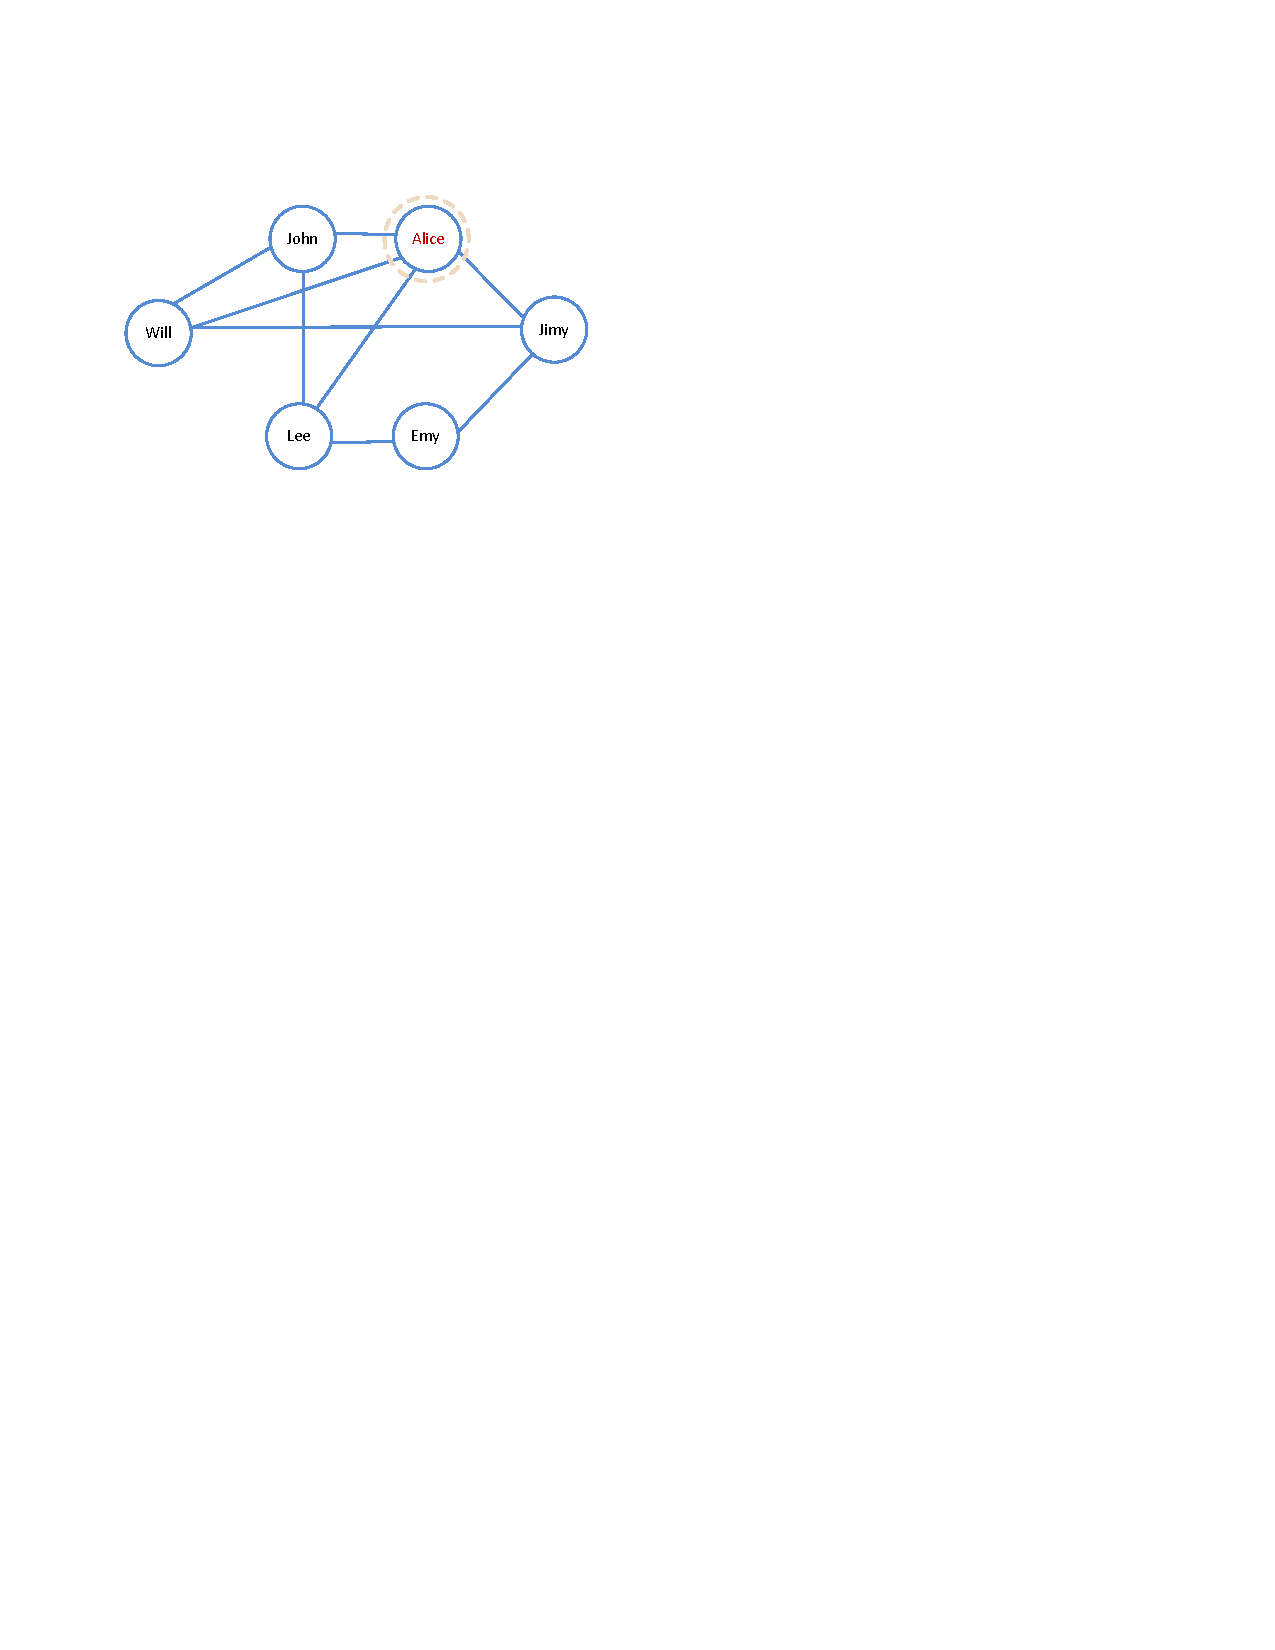
\includegraphics[width=0.5\textwidth]{Chap2-Fig1.pdf}
  \end{tabular}
  \caption{A sample social graph, individuals are represented with nodes (circles), and individuals who know each other are connected with edges (lines).}
\end{center}
\end{figure}

Social networks exhibit the small world phenomenon that node encounters are sufficient to build a connected relationship graph. The graph is a convenient tool to represent the relational structure of social networks in a natural manner, which is generally called social graph. As an example, consider a set of individuals on a social networking site where we want to find the most influential individual. Each individual can be represented using a $node$ (circle) and two individuals who know each other can be connected with an $edge$ (line). In Fig. 2.1, we show a set of six individuals and their friendships. Consider a hypothetical social theory that states that "the more individuals you know, the more influential you are." This theory in our graph translates to the individual with the maximum degree (the number of edges connected to its corresponding node) being the most influential person. Therefore, in this network Alice is the most influential individual because she knows four others, which is more than anyone else. This simple scenario is an instance of many problems that arise in social networks, which can be solved by modeling the problem as a social graph.

Any social graph contains both a set of objects, called nodes, and the connections between these nodes, called edges. Mathematically, a social graph $G$ is denoted as pair $G(V,E)$, where $V$ represents the set of nodes and $E$ represents the set of edges.

\subsection{Community}\label{Chap2_01_02}
%\esubsection{Community}
Broadly speaking, a real-world community is a body of individuals with common economical, social, or political interests/characteristics, often living in relatively close proximity. A virtual community comes into existence when like-minded users form a link and start interacting with each other. At the same time, users actively participate in activities such as data sharing and these various activities reflect their social life, giving evidences to recognize changing social community structures~\cite{LTang2011}. In other words, formation of any community requires (1) a set of at least two nodes sharing some interest and (2) interactions with respect to that interest. Therefore, a community is a structural subunit (which can be represented as a set of individuals) of a social network with high density of internal links~\cite{FLi2009}. Individuals have more social connections with other individuals inside their own community than with individuals outside. The social connections may be family, friends, common location, or common interest, which are decided by the social graph. In general, the community formation and structure has significant impact on user's mobility patterns and thus is beneficial for choosing the appropriate forwarding path.

Social community formation and structure has been studied from different perspectives such as: physical location, social relationship, interest similarity and social participation~\cite{DZhang2011}\cite{EGBoix2011}, and is thus categorized accordingly. Examples of geographic based community creation systems are Urbiflock~\cite{EGBoix2011} and MobilisGroups~\cite{RLubke2011}.  Urbiflock supports dynamic user group creation based on user profiles and physical contact proximity. Users can semantically postulate boundaries to create groups using mobile phones or smart devices. MobilisGroups is a location based group creation service, and each created group is tied to a specific location. On the other hand, Cluestr~\cite{RGrob2009}, ADESSO~\cite{SBMokhtar2010} and the work by Gao {\it et al.}~\cite{WGao2012} are some examples of social-based community creation systems. Cluestr leverages contacts from personal social networks to create groups. It aims to enable efficient initiation of group communication from nodes. In a similar way, ADESSO supports opportunistic social networking based on a set of self-organizing brokers. The proposed approach in~\cite{WGao2012} selects relays according to their capabilities, measured by social-based metrics, for forwarding data to the destination nodes. Their design of social-based metrics exploits social community and node centrality to ensure the achievement of required data delivery ratio within the given time constraint.

There are dynamic community creation mechanisms which are able to gradually form mobile social communities based on opportunistic encounters. According to Zhang {\it et al.}~\cite{DZhang2011}, their proposed method called SOCKER provides several community creation metrics and policies to realize the goal of forming different social activities, by means of dynamically creating communities in a way that produces high community completion ratio as well as high user social satisfaction. In distributed systems there are also cases where the event forwarding decisions are not based on the detected communities~\cite{NVastardis2013}. However, in many of them the existence of the communities is assumed and even more, it is regarded as an absolute necessity for the success of the proposed routing scheme. A typical example is SocialCast, presented by Costa {\it et al.}~\cite{PCosta2008}. For the employment of a publish-subscribe system in the network, the routing metrics used are co-location with other nodes sharing common interests and change in degree of connectivity, meaning the changes that took place in the physical set of neighbor nodes. However, the clear assumption made was the underlying network organized in communities. The results were taken using a distinctive mobility model called the community-based mobility model~\cite{MMusolesi2004}.

In addition to the above mentioned community formation and detection algorithms, large body of existing work focuses on community tracking which is the natural extension of community detection making it possible to observe how communities grow, shrink, merge or split with time. This method is based on the construction of temporal network representing the relationships among communities at every defined time slot. Moreover, significant dissimilarities between partitions close in time may appear in this approach, which results in artifactual community structure evolution~\cite{BMitra2012}. Community Update and Tracking algorithm (CUT)~\cite{HSMa2013} is one of the community tracking algorithms, designed to efficiently update and track the community formation and detection algorithm. According to their evaluation results, this approach can quickly and efficiently update the community structure in comparison to some other relevant algorithms. The work by Lin {\it et al.}~\cite{CXLin2010} presented the importance of tracking popular events or topics that evolve over time in the community. They proposed Popular Event Tracking algorithm (PET) that tracks the popularity of events and content revolution of the events showing the influence of community structure, interest and topic similarity to handle all the constraints. However, this proposal does not consider the mixture of multiple events.

\subsection{Centrality}\label{Chap2_01_03}
%\esubsection{Centrality}
Centrality defines how important a node is within a network. In order to identify the various types of central nodes in a network, it is important to measure degree, eigenvector, betweenness and closeness centralities. Here, we give a brief introduction about each of them.\\
\emph{Degree Centrality:} In real-world interactions, we often consider people with many connections to be important. Degree centrality transfers and defines the same idea into a measure. The degree centrality measure ranks nodes with more connections higher in terms of centrality. The degree centrality $C_d$ for node $V_i$ in a social graph is:
\begin{equation}
C_d(V_i)=d_i,
\end{equation}
where $d_i$ is the degree (number of adjacent edges) of node $V_i$. Degree centrality identifies the most active nodes in the network. A node with high degree
centrality maintains a large number of links to others. \\
\emph{Eigenvector Centrality:} Eigenvector centrality tries to generalize degree centrality by incorporating the importance of the neighbors. To keep track of neighbors, it is possible to use the adjacency matrix $A$ of a graph. Let $C_e(V_i)$ denote the eigenvector centrality of node $V_i$. We want the centrality of $V_i$ to be a function of its neighbors' centralities. Hypothetically, it is proportional to the summation of their centralities,
\begin{equation}
C_e(V_i)=\frac{1}{\lambda}\sum_{j=1}^N A_{j,i}C_e(V_j),
\end{equation}
where $\lambda$ is some fixed constant.\\
\emph{Betweenness Centrality:} Another way of looking at centrality is by considering how important nodes are in connecting other nodes. One approach, for a node $V_i$, is to compute the number of shortest paths between other nodes that pass through $V_i$,
\begin{equation}
C_b(V_i)=\sum_{s\neq t\neq V_i}\frac{\sigma_{st}V_i}{\sigma_{st}},
\end{equation}
where $\sigma_{st}$ is the number of shortest paths from node $s$ to $t$ (also known as information pathways), and $\sigma_{st}V_i$ is the number of shortest paths from $s$ to $t$ that pass through $V_i$. In other words, we are measuring how central $V_i$'s role is in connecting any pair of nodes $s$ and $t$. This measure is called
betweenness centrality.\\
\emph{Closeness Centrality:} In closeness centrality, the intuition is that the more central nodes are, the more quickly they can reach other nodes. Formally, these nodes should have a smaller average shortest path length to other nodes. Closeness centrality is defined as:
\begin{equation}
C_c(V_i)=\frac{1}{\bar{l}_{V_i}},
\end{equation}
where $\bar{l}_{V_i} = \frac{1}{n-1}\sum_{V_j \neq V_i} l_{i,j}$ is node $V_i$'s average shortest path length to other nodes. The smaller the average shortest path length, the higher the centrality for the node.\\

\subsection{Similarity}\label{Chap2_01_04}
%\esubsection{Similarity}
Similarity~\cite{EDaly2007} is a measure of the common features of a group of nodes such as background, interests, and locations. Similarity is usually referred to as homophily~\cite{MMcpherson2001}, which comes from the observation that individuals often befriend others who have similar interests and perform similar actions. Therefore, high similarity between nodes always implies the existence of a social relationship between them. For example, if two people have one or more other collaborators in common, there is a heightened probability of them being in co-operation in a partner network~\cite{DLiben-Nowell2007}. The higher the similarity that a node and the destination share, the more the opportunities that they have to encounter. Nodes with higher similarity can be good candidates for data management techniques such as replication and load balancing.

\section{User Mobility}\label{Chap2_02}
\esection{User Mobility}

With the advancement of smart phones and wireless technology, the movement of users cannot be discovered directly and can be detected by analyzing the data of daily activities such as user mobility traces and location information. This phenomenon is referred to as context awareness. Context awareness is a property of mobile devices and deals with adaptation of computing mechanisms to the current context of users. Capturing user context is an interesting research field, and several capturing approaches have been proposed in the past~\cite{IRoussaki2012}\cite{QWang2013}\cite{CAnagnostopoulos2011}. For example, context has been studied in areas such as user location~\cite{MdARahman2011}. Therefore, studying of user's collective mobility turn out to be one of the most essential aspects of social context-aware computing~\cite{WRichards2009}\cite{PMakris2013}. Mobility patterns of users' device play an important role in a wide range of mobile computing applications, such as data gathering, availability, dissemination/forwarding, and content sharing. A great interest in mobility models has been under active research in the past few years and demonstrated by~\cite{SKosta2014}\cite{RJLa2012}\cite{QDong2012}\cite{JBoudec2005}\cite{KFlorkey2011}\cite{DLe2006} including for very specific situations like pervasive conference environments. Several times, rather than moving individually people tend to move in groups. For example, participants attending a conference/meeting or students attending lectures.

However, such groups may change their movement behavior dynamically or frequently and of different strengths. People may stay longer among several groups at the same time or even in different groups at different times. Therefore, tracing real user movements' behavior can be quite heterogeneous and challenging. In order to address such challenges, numerous human mobility models have been proposed in recent years~\cite{VBorrel2009}\cite{MMusolesi2007}\cite{YXia2013}\cite{SFernandes2012}\cite{AMei2009}\cite{KLee2009}\cite{CZhao2010}.

Among the existing models, we focus on nomadic community and reference point group mobility model because they fit for modeling ad-hoc social network applications. Nomadic Community Mobility Model~\cite{AGainaru2010} was created with an inspiration from the movement pattern of a member of group of people who have no fixed home, known as nomadic societies. In this category of mobility model, nodes are moving in a random manner around the same point until the reference point changes the movement; all nodes move from their current locations to the new reference point when the reference point moves. After the group settled at the new area, nodes continue moving randomly around the new reference point until the next movement or migration. This model appropriately fits to several scenarios such as conference, museum or a military operation. Gerla {\it et al.}~\cite{MGerla2003} illustrated the use of reference point group mobility in a few representative cases. From all the cases, the interaction between exhibitors and attendees is modeled by convention scenario. In separate but networked rooms, a number of research groups give demos of their findings such as products or projects. While a number of attendees move from room to room in a group, they may stop in one room for some time and then move on to another. They may also just quickly pass through one room. This is referred to as the convention model.

Tracking users' and predicting their future movement behavior regularly have been interesting but challenging topic in recent years. User tracking and mobility prediction abilities can be used in various application scenarios such as pervasive conference systems. Knowing the users' mobility behaviors, predicting user recent future locations, stay durations and next contacts as a friendship are crucial issues~\cite{PPirozmand2014}. In order to succeed in predicting user mobility, it is important to investigate personal and environmental factors. Predicting users' recent future locations, time and the individual going to be contacted frequently has many things to do with ASNET applications such as data dissemination in pervasive conference systems. Hence, mobility traces of users have been widely examined in order to gain knowledge about humans' mobility patterns and forecast their future locations~\cite{AAsahara2011}, time~\cite{DTMT2012} and contacts~\cite{HANguyen2012} more accurately.

To accurately predict user's location, it's crucial to distinguish and characterize mobility information of users in ASNET application scenarios like social events. Some existing researches such as~\cite{PHui2005}\cite{AChaintreau2007}\cite{TKaragiannis2010}, indicate that user mobility pattern is always characterized by the distribution of inter-contact time between users. However, they identified that the periodical association/re-affiliation within several communities as user mobility, and then examined the distribution of user sojourn time in communities instead. According to Du {\it et al.}~\cite{YDu2011}, Sojourn time is defined as the user contact duration in a geo-community. This user contact duration remarks on user mobility and contact opportunity in MSNs. A user will be considered to forward data between geocommunities if its average sojourn time is shorter that allows it to move in the network frequently. The knowledge of user mobility information is essential to design data management protocols in ASNETs.

When we see the human mobility pattern on the other hand, almost all the anticipated ASNET application scenarios are tightly coupled with humans' moving behaviors. The reason behind this logic is that wireless devices are generally carried by humans and are governed by their daily activities~\cite{DKotz2005}\cite{CGonzalez2008}\cite{CSong2010}. Human daily activities are regulated by their associated societal, cultural and environmental duties and very challenging to predict upon diversified locations and times. Moreover, it is still not clear how to postulate the complicated human mobility using the available mobility modeling, which, however, is essential to design the challenging and most important protocols. The design of data and resource management protocols requires understanding of human movement and pattern habits of their connectivity (frequency of meetings, frequency of visiting locations, average duration of contact, etc.).

\begin{figure}[b]
\begin{center}
  \begin{tabular}{c}
  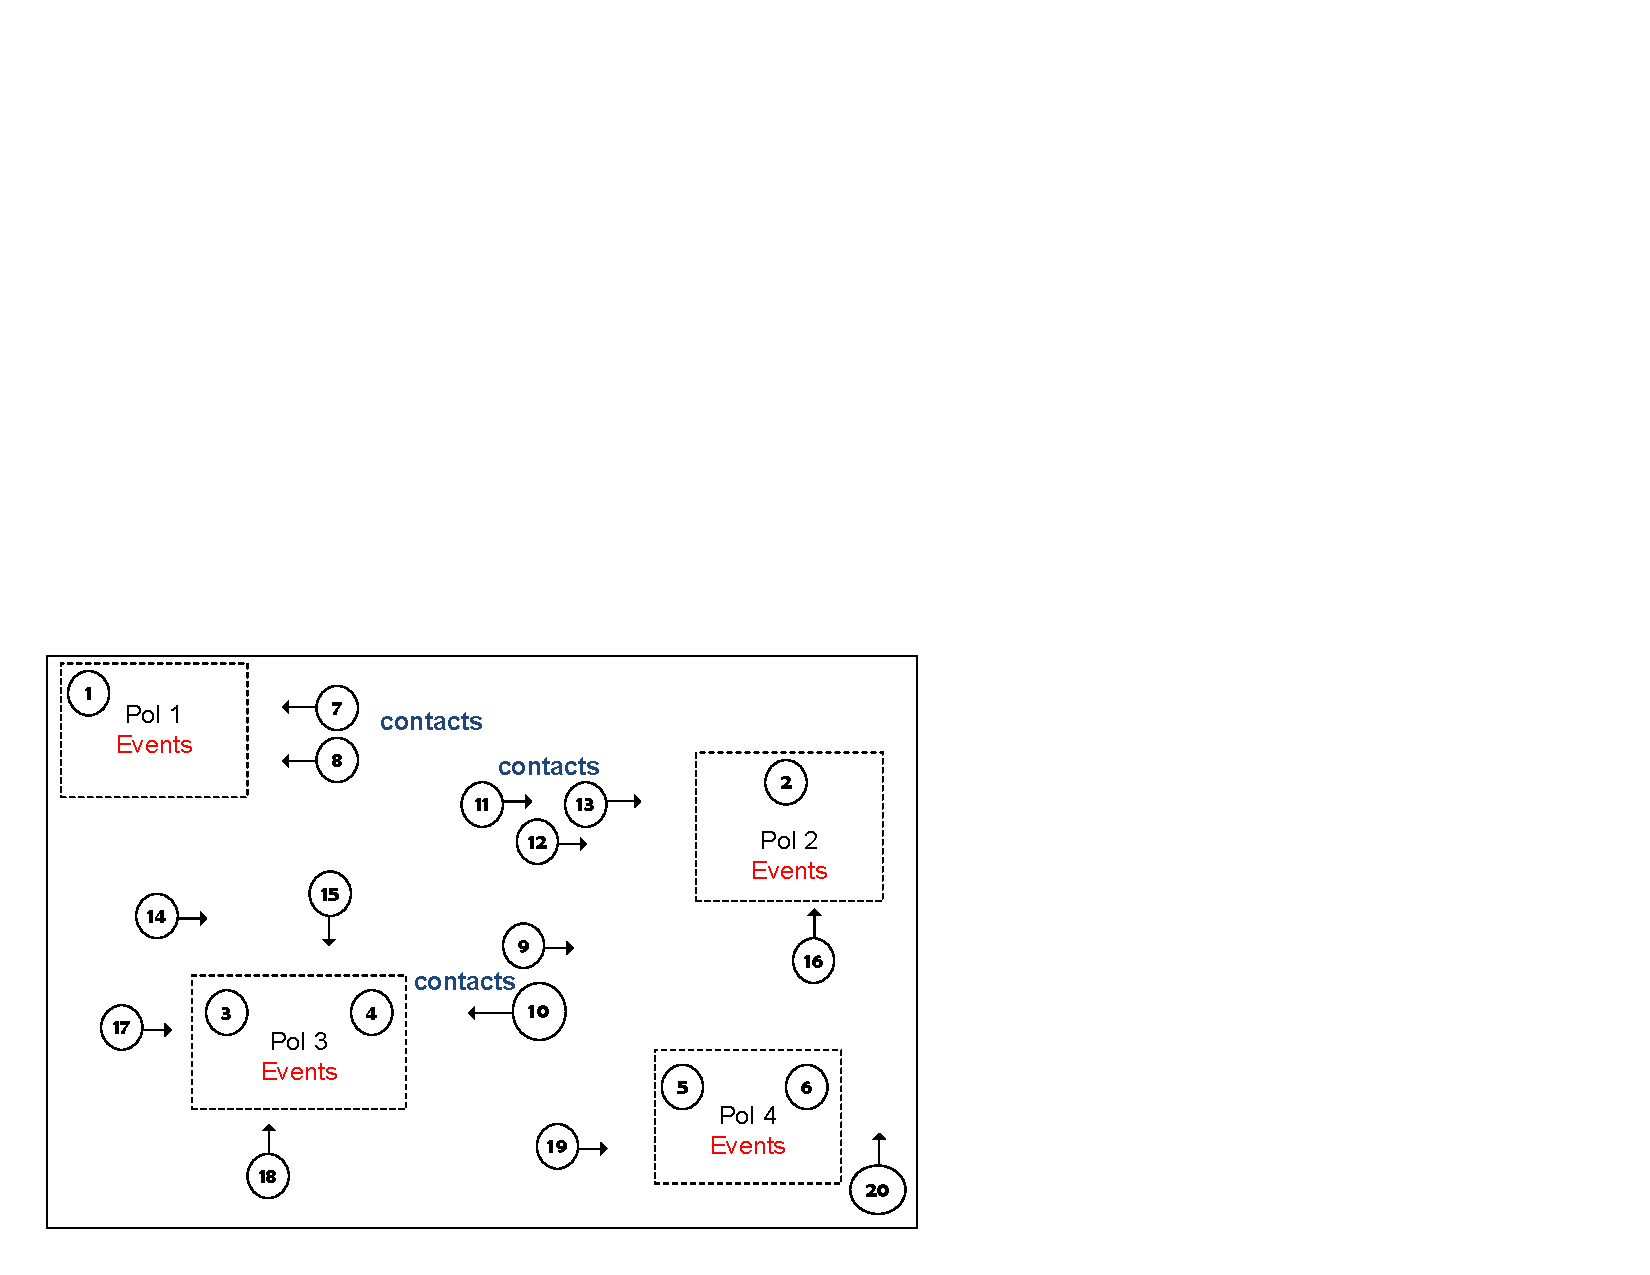
\includegraphics[width=0.6\textwidth]{Chap2-Fig2.pdf}
  \end{tabular}
  \caption{PoIs and mobile users (participants in the same smart environment).}
\end{center}
\end{figure}

Therefore, there is challenge in studying human mobility and, specifically to data management where ASNETs are more applicable. As discussed by Karamshuk {\it et al.}~\cite{DKaramshuk2011}, the emerging main dimensions of people's movements are categorized as spatial, social and temporal axes. At the same time there were researchers who demonstrated their framework. For example: Xie {\it et al.}~\cite{RXie2011} designed a framework of individual mobility pattern mining. They demonstrated their framework by using real data set containing mobile phone data. Based on the result of an experiment conducted over real data, they have shown that their framework is efficient in discovering individual mobility patterns that can be used for wide applications. In order to represent the space and time contexts in ad-hoc network services, the work in~\cite{NYu2013} adopted concept of Point of Interests (PoIs). PoIs are popular places in the navigation system, and users who are inside PoI can get events happening or being announced in the PoI. They assume that each user has a unique user id, a mobility profile with a series of contacts and PoI visits, a set of PoI events the user attended with time of the event, and a user influence lifetime TL to specify the time duration the user is willing to share the event with other users. In Fig. 2.2 there are four PoIs (denoted using rectangles) and twenty nodes/mobile users (denoted using circles), where some users are moving outside PoIs (moving directions are represented using arrows). Mobile users may visit the PoIs at different times and can be attracted by the events during their stays inside the PoIs. Later, they can further influence other mobile users with the PoI events via their mobile devices when they meet other friends/users outside the PoIs any time before the expiration of their influence lifetimes. Once a user outside its PoI receives the event information, it may be further forwarded to other users. Therefore, the information influence is continued and connected in a ripple carry fashion.

\section{Middleware Solutions}\label{Chap2_03}
\esection{Middleware Solutions}
In this section, we discuss ASNET middleware design models with adherent solutions. Specifically, it will be discussed how services like data dissemination can be achieved using publish/subscribe, mobile cloud and social-based approaches. We classify the middleware for MANETs in the following way, as depicted in Fig. 2.3. Note that the approaches we discuss are mainly targeted to the socially-aware middleware and hence will not necessarily apply to middleware in which the design does not consider social behaviors.

\begin{figure}[t]
\begin{center}
  \begin{tabular}{c}
  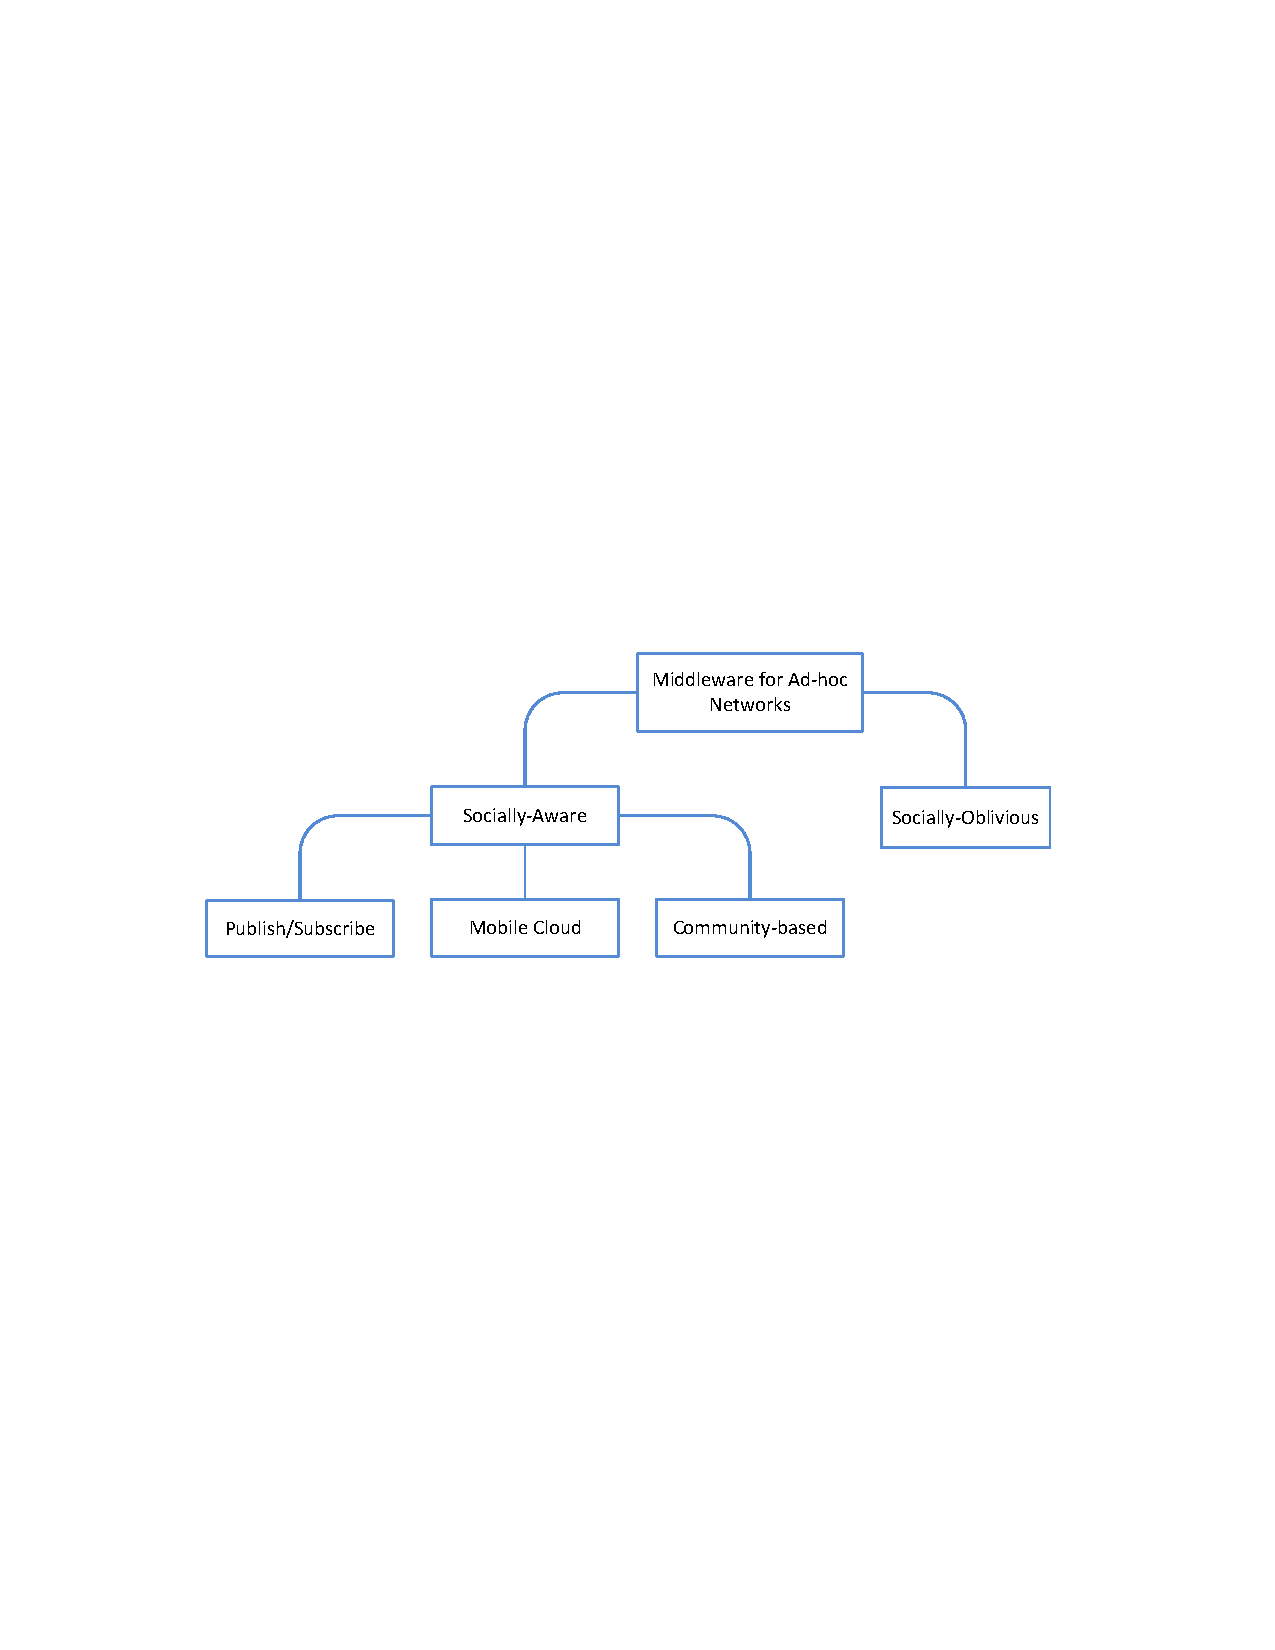
\includegraphics[width=0.85\textwidth]{Chap2-Fig3.pdf}
  \end{tabular}
  \caption{Categorization of ad-hoc networking middleware.}
\end{center}
\end{figure}

\subsection{Publish/Subscribe}\label{Chap2_03_01}
\esubsection{Publish/Subscribe}
While communication via wireless connection is more flexible than wired ones, it is often not robust, and the coverage is not always broad. Therefore, it is important to give a presentation on a socially-aware ad-hoc network middleware design approach using publish/subscribe concepts. Dynamic network topology and limited resources in ASNETs make the implementation of publish/subscribe middleware designed for infrastructure social networks unsuitable for this network paradigm. Some existing publish/subscribe communication schemes in MANETs are designed for specific scenarios and are not adaptive enough to be used in different socially-aware ad-hoc network scenarios.

The publish/subscribe (Pub/Sub) paradigm recently emerges as a promising solution to data dissemination owing to the decoupling characteristic. It has attracted a lot of attention from many research works. In such systems, loose-coupling is achieved by simply having producers publish information into the network without knowing the identity, location, and number of subscribers. Likewise, consumers subscribe to specific information without knowing the identity, location, and number of publishers~\cite{AKYCheung2010}\cite{EYoneki2007}. On the other hand, data dissemination systems should take care of both network and device resource constraints~\cite{CBoldrini2008}. Most approaches over publish/subscribe in the literature provide users with three primitives over information items. For instance, in Xia {\it et al.}~\cite{FXia2013} the service primitives are publishing, subscribing and brokering. Publish is used by information producers to announce the availability of an information item to the network. Subscribe is used by information consumers to express their interest in receiving information item. Users can subscribe to either specific items or scopes of the available information in the network. The broker is the interface between the publisher and subscriber which provides routing, event matching, filtering services, etc.

\begin{figure}[t]
\begin{center}
  \begin{tabular}{c}
  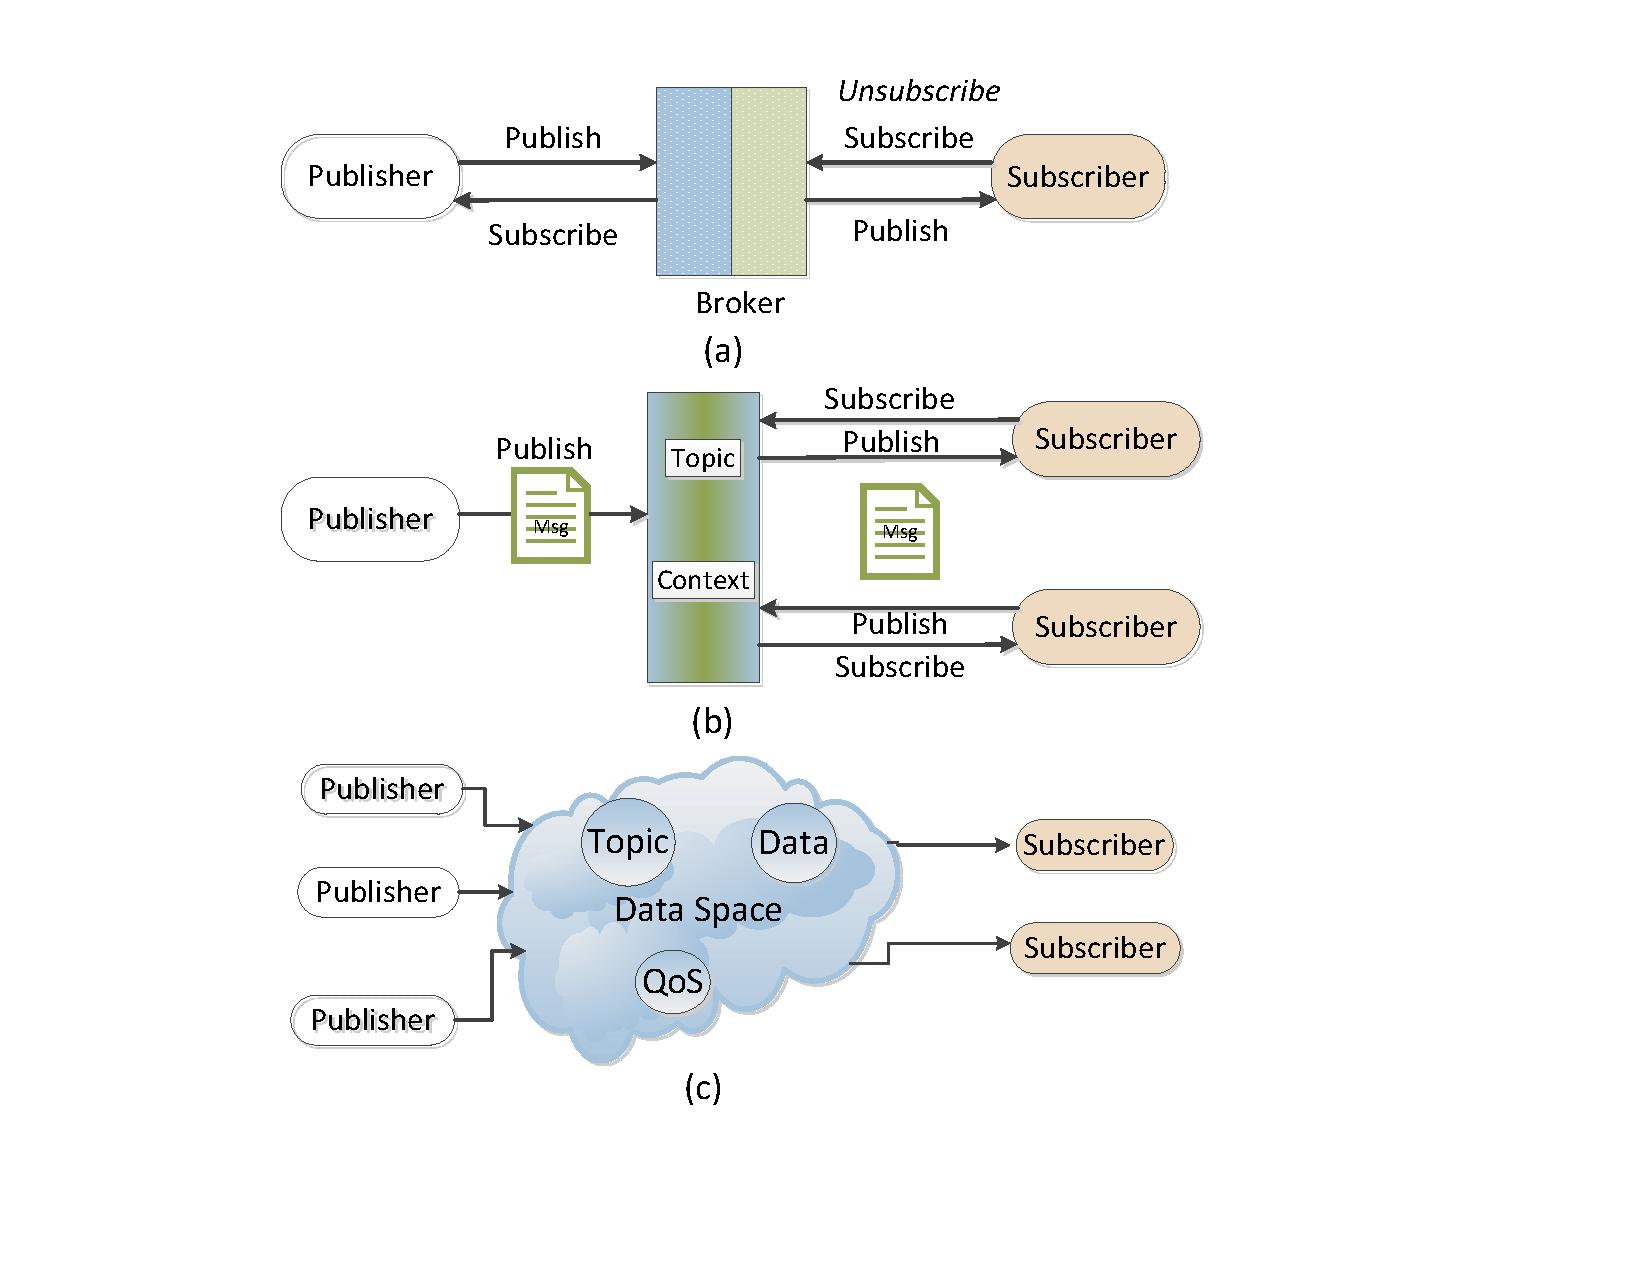
\includegraphics[width=0.6\textwidth]{Chap2-Fig4.pdf}
  \end{tabular}
  \caption{Sample message communication models: a) abstract view of the primitives in publish/subscribe model. b) models of publishing and subscription type (topic-based, context-based or attribute-based). c) social data storage on a cloud.}
\end{center}
\end{figure}

Additionally, publish/subscribe message oriented middleware forms on asynchronous mode and enables data-centric communications in which customers subscribe to the data they need and publishers make this data available. Typically messages are published to a broker on well-known topics by publisher clients, and the subscription on topics is made by subscriber clients as shown in Figs. 2.4(a) and (b).The broker also gives guarantees of delivery, so a message is not deleted until all subscribers to a topic have received the message from the broker, relieving the sender from the burden of ensuring delivery.

Clearly, most of the existing message communication systems cannot be handled according to the conventional network paradigms, which are not able to accommodate the scale, heterogeneity and complexity of such services. Novel paradigms such as spontaneous networks and ASNETs are needed for designing and managing these communication services. Spontaneous networks are dynamic collaborative networks stemming from the impromptu interaction of mobile or fixed devices, administered by typically small groups of socially interacting users. To accelerate this type of ad-hoc networking adoption, in particular, Bellavista {\it et al.}~\cite{PBellavista2012} designed a Real Adhoc Multihop Peer-to-peer (RAMP) middleware for flexible, dynamic and application-driven spontaneous network management that fulfills differentiated application requirements while coping with heterogeneity and dynamistic. While such applications can be developed from scratch, programming support from a middleware or framework can improve the productivity of developers significantly, as well as the performance and features of the applications.

Some of the very few and most prominent solutions that target publish/subscribe event dissemination are: MobiClique~\cite{AKPietilainen2009} and SocialCast~\cite{PCosta2008}. In an approach by Pietilainen {\it et al.}~\cite{AKPietilainen2009}, introducing a middleware called MobiClique, the utilization of publish/subscribe system is presented. MobiClique is able to form and preserve a mobile ad-hoc social network, providing content exchange by exploiting the user mobility. However, it lacks the ability to predict user contacts and therefore performs a form of flooding as a means of content dissemination, leading to low efficiency and very high resource usage. As a general idea though, it may provide a valuable insight on how publish/subscribe systems will be in the near future. SocialCast is another interesting system in this category that attempts to exploit social information in publish/subscribe service for the first time. It assumes that users with common interests tend to meet with each other more often than with other users. Taking shared interests of users into account, data forwarding in the SocialCast can be achieved not only based on social ties and mobility patterns, but also by the interest of destination nodes. A drawback of this method is that it works well when all members of each community are interested in the same type of content, but it is not clear how it works for higher number of interests.

In addition to the above two middleware solutions, the authors in~\cite{EYoneki2007} introduce a novel approach for building a backbone for publish/subscribe communication system based on uncovered community structure. In this work, distributed community detection from the real trace is exploited to propose a socio-aware overlay over detected communities. The implementation of community detection is implemented by gossiping when users are in contact to each other. Brokers in this system are certain users that form the overlay and have high centrality values in the community. During data interchange, information such as subscription and centrality values are exchanged with time stamp attached. The subscription list is moved from the old to the new broker when the closeness centrality of this broker changes and updated information is sent to all the brokers in the community. While gossiping, subscription information is broadcasted to the brokers. When the broker receives the publication, it propagates to all other brokers and then the broker checks its own subscription information. However, this work does not explore various centrality characteristics such as betweenness centrality for filling the gap between two communities.

Socially-aware applications and services have leveraged out-of-band social relationships for various objectives such as improving security, inferring trust, providing incentives for resource sharing, and building overlays for private communication. For the design of ASNET middleware, it is important to know that all such applications use social data of users, collected and managed in the form of a social graph within an application domain. A user's social data, which consists of the user's direct relations with other users in the applications social graph, could be stored on systems with various types of architectures.


\subsection{Mobile Cloud}\label{Chap2_03_02}
\esubsection{Mobile Cloud}
Except very few works such as by Huang {\it et al.}~\cite{DHuang2010} who proposed MobiCloud that enhances the operation of ad-hoc network itself by treating mobile nodes as service nodes, it was almost impossible to consider cloud solutions for ad-hoc networks because of the networks resource constrained nature in which the link must be over a high-bandwidth 3G/4G/LTE network. However, recent years have witnessed two important trends that pose new requirements to serve the network with cloud computing solutions. The first trend is the emergence of MCS and the ever increasing number of sensing and responding applications that familiarize their behavior to social properties of users, based on continuous readings from sensors. The second trend is the emergence of mobile cloud (puts cloud into pocket)~\cite{NFernando2013}. These two trends open the issue to consider mobile cloud solution (by applying different issues for mobile devices to achieve energy saving) for ASNETs.

Furthermore, the popularity of socially-aware applications and the commensurate rise in scalability and privacy concerns have motivated a number of proposals for designing effective middleware that do not require users to give up their data to any particular (potentially untrustworthy) provider. The proposed approach is to use mobile cloud-based hosting services to store social data as shown in Fig. 2.4(c). For instance, Contrail~\cite{PStuedi2011} is a mobile device-centric social network that leverages a store-and-forward service hosted in the mobile cloud to relay encrypted data to and from users. ASNETs reveal users' content consumption to their peers who host the content which is particularly a serious problem for systems like Contrail, unless they have a "push" architecture where users always download accessible content, whether they view it or not, which is highly inefficient. Fernando {\it et al.}~\cite{NFernando2013} proposed an architecture for implementing a mobile cloud in a resource constrained environments like ASNETs. To facilitate the development of such technologies, we need to research the unique set of challenges for mobile cloud computing.

\subsection{Social-based}\label{Chap2_03_03}
\esubsection{Social Community-based}
This approach exploits information about users' social behavior based on the movement of nodes in the community and the structure of the community itself. For example: Fan {\it et al.}~\cite{JFan2013} design a middleware to address data dissemination from a single super-user to other users among several communities and proposed an efficient super-user route to broadcast data actively. They introduced the concepts of geocommunity and geocentrality into mobile social networking. A semi-Markov process is proposed in their work to model user mobility based on the geographic regularity of human mobility and geocentrality as the super-user among communities. However, the way how community structure is conducted from a social graph and application of mobility model varies a lot among designers and researchers.

Another known example in this category is a system called ContentPlace~\cite{CBoldrini2010}. It is a social-based data dissemination system that forwards data based on defined community-based relay selection policies. Moreover, it employs the same community detection mechanisms as used in the socio-aware overlay approach~\cite{EYoneki2007}. In ContentPlace, social characteristics of the users are exploited to select data object encounter users exchange. In order to accomplish this task, a utility function for every data object is provided. The utility value of all the data objects in their local buffer is calculated by the encounter users to exchange data. After this, the set of data objects that maximizes the local utility of its cache are selected considering the resource constraints.

Although, most of the existing community detection algorithms are centralized, community detection and formation plays an important role in the design of social-based routing schemes. BUBBLE Rap~\cite{PHui2011} is an interesting work that uses weighted network analysis and k-clique algorithms for community detection in a decentralized fashion from a diverse set of real world traces. However, its evaluation does not focus on hierarchical community structure because of the limited size of available mobility traces. We thus need to investigate the substantial amount of prior research as well as availability of data on general social-based algorithms in order to design effective and novel social-based data management or delivery schemes.

Table 2.1 summarizes the representative protocols for the above discussed three approaches and their evaluation based on list of social behaviors.
\begin{table}\fontsize{7.8}{10}\selectfont
\centering
\caption{Summary of existing middleware/prtocols in terms of their choice of social behaviors used}
\renewcommand{\arraystretch}{2.3}
\begin{tabular}{|c|c|c|c|c|c|c|c|}
\hline
\multicolumn{1}{c}{{Protocols}} & \multicolumn{1}{c}{{Approach}} & \multicolumn{1}{c}{{Community}} & \multicolumn{1}{c}{{Friendship}} & \multicolumn{1}{c}{{Movement Pattern}} & \multicolumn{1}{c}{{Similarity}} & \multicolumn{1}{c}{{Centrality}} & \multicolumn{1}{c}{{Link Prediction}}\\
\hline
\multicolumn{1}{c}{RAMP~\cite{PBellavista2012}} & \multicolumn{1}{c}{Publish/Subscribe} & \multicolumn{1}{c}{\checkmark} & \multicolumn{1}{c}{$\times$} & \multicolumn{1}{c}{\checkmark} & \multicolumn{1}{c}{$\times$} & \multicolumn{1}{c}{$\times$} & \multicolumn{1}{c}{-}\\
\multicolumn{1}{c}{MobiClique~\cite{AKPietilainen2009}} & \multicolumn{1}{c}{Publish/Subscribe} & \multicolumn{1}{c}{\checkmark} & \multicolumn{1}{c}{\checkmark} & \multicolumn{1}{c}{\checkmark} & \multicolumn{1}{c}{-} & \multicolumn{1}{c}{$\times$} & \multicolumn{1}{c}{$\times$}\\
\multicolumn{1}{c}{SocialCast~\cite{PCosta2008}} & \multicolumn{1}{c}{Publish/Subscribe} & \multicolumn{1}{c}{\checkmark} & \multicolumn{1}{c}{$\times$} & \multicolumn{1}{c}{\checkmark} & \multicolumn{1}{c}{$\times$} & \multicolumn{1}{c}{$\times$} & \multicolumn{1}{c}{\checkmark}\\
\multicolumn{1}{c}{MobiCloud~\cite{DHuang2010}} & \multicolumn{1}{c}{Mobile Cloud} & \multicolumn{1}{c}{-} & \multicolumn{1}{c}{-} & \multicolumn{1}{c}{\checkmark} & \multicolumn{1}{c}{$\times$} & \multicolumn{1}{c}{$\times$} & \multicolumn{1}{c}{$\times$}\\
\multicolumn{1}{c}{Contrail~\cite{PStuedi2011}} & \multicolumn{1}{c}{Mobile Cloud} & \multicolumn{1}{c}{$\times$} & \multicolumn{1}{c}{\checkmark} & \multicolumn{1}{c}{$\times$} & \multicolumn{1}{c}{\checkmark} & \multicolumn{1}{c}{$\times$} & \multicolumn{1}{c}{$\times$}\\
\multicolumn{1}{c}{GeoCommunity~\cite{JFan2013}} & \multicolumn{1}{c}{social-based} & \multicolumn{1}{c}{\checkmark} & \multicolumn{1}{c}{$\times$} & \multicolumn{1}{c}{\checkmark} & \multicolumn{1}{c}{\checkmark} & \multicolumn{1}{c}{\checkmark} & \multicolumn{1}{c}{$\times$}\\
\multicolumn{1}{c}{ContentPlace~\cite{CBoldrini2010}} & \multicolumn{1}{c}{social-based} & \multicolumn{1}{c}{\checkmark} & \multicolumn{1}{c}{$\times$} & \multicolumn{1}{c}{\checkmark} & \multicolumn{1}{c}{$\times$} & \multicolumn{1}{c}{$\times$} & \multicolumn{1}{c}{$\times$}\\
\multicolumn{1}{c}{BUBBLE Rap~\cite{PHui2011}} & \multicolumn{1}{c}{social-based} & \multicolumn{1}{c}{\checkmark} & \multicolumn{1}{c}{$\times$} & \multicolumn{1}{c}{\checkmark} & \multicolumn{1}{c}{\checkmark} & \multicolumn{1}{c}{\checkmark} & \multicolumn{1}{c}{$\times$}\\
\hline
\multicolumn{8}{c}{("\checkmark" if the middleware/protocol satisfies the feature, "$\times$" if not and "-" for ambiguous cases)}\\
\end{tabular}
\end{table}

\section{Data Replication}\label{Chap2_04}
\esection{Data Replication}

\subsection{Data Replication in Social Networks}\label{Chap2_04_01}
\esubsection{Data Replication in Social Networks}
Recently, there has been a recent unprecedented increase in the use of social networks and applications with a social component. Since highly scalable and elastic network resources are required to deploy new social applications, it is promising to deploy social applications in the cloud~\cite{PStuedi2011}\cite{ZWang2012}. When placing social networks data among multiple clouds, it maintains the social locality (i.e., one-hop locality) by replicating the data of a user's every neighbor to the cloud that hosts the user's own data~\cite{Pujol2010}\cite{DTran2012}\cite{FBenevenuto2009}, which has been shown to be necessary for social network services due to the data access pattern that a user's most activities happen between herself and her neighbors (e.g., all friends must be accessed to collect their recent tweets for a Twitter user). Maintaining social locality eliminates the inter-cloud multi-get traffic and the an unpredictable response time because all the data requested by a user can be retrieved from a single cloud. Compared with full replication, the storage cost is much lower because only neighbors need to be replicated across clouds.

In a social network system, contents distribute among users by users sharing them. A number of research efforts have been devoted to studying content dissemination in social network applications. Kwak {\it et al.}~\cite{HKwak2010} investigated the impact of users' re-tweets on data diffusion in Twitter. An alternative social network system stores social information on users' mobile devices, as proposed in~\cite{AKPietilainen2009}. Pujol {\it et al.}~\cite{Pujol2010} have investigated the difficulties of scaling online social network, and designed a social partitioning and replication middleware in which users' friends can be co-located in the same server. Tran {\it et al.}~\cite{DTran2012} have studied the partition of contents in the online social network by taking social relationships into consideration. Cheng {\it et al.}~\cite{XCheng2011} have studied the partitioning schemes for social contents to achieve a balanced load at the servers and preserve the social relationships.

Mobile social networks originate from online social networks which emphasize the relationship of similar interests or commonalities. Social opportunistic networks are based mainly on the prediction of contact opportunities and concentrate on the social relationships between mobile nodes and their regular movements~\cite{FXia2013}. Vehicle social networks consider the social properties of vehicles and passengers. For example, the work by Zhou {\it et al.}~\cite{LZhou2011} study the distributed heterogeneous media service scheme that jointly solves the content dissemination, cache update and fairness problems. Guo {\it et al.}~\cite{BGuo2013} introduced a new feature to mobile social computing middleware, cross community mining, which discovers the implicit semantics of a public place as derived from social activities in both online and ad-hoc physical communities and in spontaneous interaction opportunity recommendations based on the place semantics to allow an ad-hoc physical community of users to engage in place-aware social interactions.

Another research work in~\cite{ANatanzon2013} indicates that data replication techniques are of two types, either host based or array based. Host-based replication systems are less desired by application users because of their maintenance difficulty. Array-based replication consists of synchronous and asynchronous replication technologies. Examples of efficient asynchronous replication algorithms are presented by Weatherspoon {\it et al.}~\cite{HWeatherspoon2009} and Yan {\it et al.}~\cite{RYan2004}. The work by Krishnamurthy {\it et al.}~\cite{SKrishnamurthy2003} proposed a system that leverages replication for maximizing data availability and reducing response time during a failure. There are some databases that use replication and load balancing to increase availability and improve performance such as the Yahoo distributed database~\cite{BFCooper2008}. However, these methods are restricted to the specific applications framework, and tolerate events where response times rise, a situation which is not acceptable in most of the current cases. Few replication mechanisms reduce latency by allowing simultaneous access to multiple storage spaces and placing data locally (e.g. the work by Sovran {\it et al.}~\cite{YSovran2011}). In fact, such systems do need application-level awareness as disaster in the network can lead to general-purpose applications inconsistency. None of the aforesaid works designates a mechanism for applying social behaviors and mobility of users in the replication process.

\subsection{Data Replication in MANETs}\label{Chap2_04_02}
\esubsection{Data Replication in MANETs}
In a network where content exchange or delivery is done by autonomous nodes, it becomes challenging to construct efficient distributed algorithms for data replication. This is due to the autonomy of the nodes and their freedom to decide which objects they want to replicate. Additionally, mobility (i.e., nodes leaving the network autonomously) poses significant challenges to data availability. A number of data replication methods have been proposed for MANETs in the literature. A survey of these protocols is given in~\cite{ADerhab2009} and~\cite{PPadmanabhan2008}. Most of these methods/protocols assume that the memory size of each node is same but in the real scenario different devices that form an ad-hoc network may consist of heterogeneous nodes having different characteristics. On the other hand, some of the proposed protocols assume that the access frequencies of devices to data items are the same at every time but similar to the above case it is not true in real scenario, in which access frequencies may be different at different times.

The proposals by Hara {\it et al.}~\cite{THara2009}\cite{THara2006} discuss replication in MANETs. E-DCG+~\cite{THara2006} creates groups of nodes that are bi-connected components, and shares replicas in larger groups of nodes to provide high stability. The work in~\cite{THara2009} aims at classifying different replica consistency levels in a MANET based on application requirements, and proposes protocols to realize them. In their work, each replica is valid till its original owner updates it. Hence, applying strict consistency updates may potentially degrade the system performance, given the inherently dynamic nature of the environment. Thus, the work assumes that all applications do not necessarily require such strict consistency, and it defines consistency based on group-level information consistency. While R3~\cite{XTie2011} is an algorithm that can cope with the dynamic nature of nodes and is based on the distribution of path delays, their model ignored integration of social properties and the effects of load. It showed replication yields significant delay gains if and only if the path delays have high unpredictability without making any other assumptions about the underlying delay distribution. Notably, these proposals~\cite{THara2009}\cite{THara2006}\cite{XTie2011} do not consider social behavior integration in to the solution.

Moreover, in a MANET, the mobile nodes move freely and disconnections take place frequently, thereby reducing the data accessibility due to the dynamically changing network topology. Huang {\it et al.}~\cite{JLHuang2006} propose a group mobility model and a replica allocation scheme to address the problem of data accessibility by replicating data items and using the concept of group mobility, where a group of mobile nodes move together. Jain {\it et al.}~\cite{SJain2013} proposed a replica allocation method called W-DCG (an extension to DCG~\cite{THara2001}), that considers node properties such as memory capacity and remaining battery power while replicating data on nodes to achieve better load-balancing. They also use dynamic access frequencies to replicate data items which are currently in demand. Classic data replication techniques~\cite{YSaito2005} use predefined and static servers, requiring reliable delivery of packets and the ordering of replication messages. However, node failures and radio obstacles exists in most of the time and places. Valuable works regarding data replication for MANETs with obstacles and node failures have been tried to be addressed by Detti {\it et al.}~\cite{ADetti2010}.

MANETs operational services, such as resource, location and distribution of connectivity information, deal with mobility and resource constraints to support the applications. According to Mannes {\it et al.}~\cite{EMannes2012}, the reliability and availability of these services can be assured by data management approaches, as replication technique using quorum systems. However, these systems are vulnerable to selfish and malicious nodes that intentionally do not collaborate with replication or spread malicious data while participating in the process of replication. They proposed $QS^2$, a bio-inspired scheme to tolerate selfish and malicious nodes in replication process of quorum systems that can effectively detect misbehaving nodes in quorum systems to increase data reliability. This work is one of the proposed protocols based on an inspiration from nature (bio-inspired), but does not consider social behaviors in their solution.

\section{Load Balancing}\label{Chap2_05}
\esection{Load Balancing}
Load balancing has been a widely explored research topic for the past two decades since the introduction of parallel and distributed computing. The goal of all load balancing solutions is to evenly distribute workload to all available resources~\cite{YZhu2013}\cite{JBalasangameshwara2013}. In addition, strategy and method of load balancing will directly affect the performance of the network system. Therefore, load balancing mechanisms should be fair~\cite{JBalasangameshwara2013}. Load balancing solutions can be found in four software layers: network, operating system, middleware, and application. The layer in which a load balancing strategy is implemented depends on which layer contains the logic to make effective load balancing decisions. For example, it would be ineffective to use a random DNS redirection strategy in the network layer or process migration in the OS layer to load balance a content-based publish/subscribe system that resides at the middleware layer. This is because these approaches cannot identify the relationship (whether it be intersecting, superset, subset, equal, or empty) between subscriptions nor estimate the load of a subscription imposed onto a broker already servicing an arbitrary set of subscriptions.

In terms of the mechanism applied to design, structure, method and partitioning of nodes participating in the network; load-balancing algorithms can be roughly categorized as tree-based, DHT-based, cluster-based and community-based. Tree-based is based on the method used to produce a spanning tree representation of the network system, particularly publish/subscribe systems (e.g., Chen {\it et al.}~\cite{HChen2010}, Zhang {\it et al.}~\cite{HZhang2008}). DHT-based approaches use specialized placement algorithms to assign responsibility for each object to specific nodes, and directed search protocols to efficiently locate objects. DHTs mostly differ in the rules they use for associating the objects to nodes, their routing and lookup protocol, and their topology (e.g., Bianchi {\it et al.}~\cite{SBianchi2006}). Load balancing algorithms in which the computing nodes are partitioned into clusters based on data transfer in the network are called as cluster-based methods (e.g., Lang {\it et al.}~\cite{WLang2010}, Kwak {\it et al.}~\cite{KKwak2009}, Jafarpour {\it et al.}~\cite{HJafarpour2009}). Community-based load balancing is done by partitioning the set of nodes into a predefined number of communities. We considered community-based load balancing approach in our work.

Despite what is commonly believed in the networking community, using multiple paths for routing messages does not necessarily balance the load better than single-path routing. Unless we use a huge number of paths, multi-path routing does not improve the load balance. Ganjali and Keshavarzian~\cite{YGanjali2004} have shown this viewpoint in their work. Cheung and Jacobsen~\cite{AKYCheung2010} proposed a dynamic load balancing scheme for content-based pub/sub system where brokers are structured in a hierarchical way. Brokers with more than one neighboring broker are referred to as cluster-head brokers, while brokers with only one neighbor are referred to as edge brokers. Publishers connect to cluster-head brokers, while subscribers are connected to edge brokers. The proposed scheme allows for two levels of load balancing: local-level where edge brokers within the same cluster load balance with each other; and global-level where edge brokers from two different clusters load balance with each other. The main drawback of this scheme is subscriptions may migrate from one broker to another which not only is an extra load on brokers, but also does not preserve subscription locality.

Unlike Cluster-based pub/sub architecture which provides transparent fault tolerance, it is not clear how the hierarchical (tree-based) architecture overcomes the broker failures. As a DHT-based pub/sub framework, Meghdoot is an interesting load balancing scheme~\cite{AGupta2004}. In Meghdoot the content space is partitioned among brokers and each broker is responsible for one of the partitions. The subscriptions are routed to and stored in the corresponding brokers for their partitions. Each publication is also routed to the broker responsible for the partition that the publication falls in. This broker is referred to as Rendezvous Point. After receiving the publication, the Rendezvous Point matches the publication with the subscriptions and routes the publication to the brokers with matching subscriptions. The overloaded brokers can offload part of their load by dividing their partition into two sections and transmit the responsibility of one section along with the corresponding subscriptions to another underloaded broker. However, this may require retransmission of subscriptions which results in extra load.

Shuffle is another DHT-based pub/sub scheme that provides load balancing~\cite{HZhang2008}. Unlike Meghdoot, in Shuffle subscriptions are stored in all brokers in the path from the subscribing broker to the Rendezvous Point. An overloaded broker exploits the replication of subscriptions and designates an underloaded broker in its children list in the dissemination tree to take the responsibility of content matching and forwarding to the subscribers in its sub-tree. This scheme relies on the fact that the path for forwarding publication is the reverse path of subscription dissemination that may not be accurate if there are failures in the broker network.

\section{User Selfishness and Incentive Schemes}\label{Chap2_06}
\esection{User Selfishness and Incentive Schemes}
Almost all the existing data dissemination and forwarding protocols assume that users are willing to help each other in data forwarding and delivery. However, network and device resources such as energy, cache and bandwidth in real applications are limited and a user might not be interested to relay messages for the other users. In other words, some users may have selfish behaviors in data relaying which could degrade the performance of socially-aware data dissemination algorithms significantly. According to Li {\it et al.}~\cite{QLi2012}, two kinds of selfish behavior can be defined for a non-cooperative users. In some cases, a selfish user wants to help other users with whom he has social relationships (e.g., friends, classmates, colleagues), because he received help from them in the past or will probably get help in the future. This kind of selfish behavior is called individual selfishness. A selfish user may show different degree of selfishness (or cooperation) to other users based on social tie strength. This behavior is also called social selfishness.

ASNET is wholly dependent on the cooperation of participating users in communication for its successful operation. The lack of a fixed infrastructure in ad-hoc networks compels users to rely on each other in order to maintain stability. But sometimes users act unwillingly and do not function as intended. There are two types of ad-hoc networks, single-hop and multi-hop~\cite{NKang2010}. Users are free to directly communicate with others in their radio range in single-hop whereas in multi-hop, users rely on others to transmit packets to respective destinations. Therefore, cooperation of users in multi-hop networks is required for its effective operation. Detecting selfish users in wireless networks is an important issue that has been drawing considerable attention. Misbehavior has been widely studied in different categories of networking such as wireless networks~\cite{JChoi2011}, mobile ad-hoc networks~\cite{PGera2011}, peer-to-peer networks~\cite{DHales2005}, vehicular networks~\cite{MRaya2007}, and delay tolerant networks~\cite{YLi2011}\cite{QLiandGCao2012}. The solutions proposed thus far have applied to reputation, incentive, ACK and game theory-based approaches. The idea is to motivate users to collaborate with others in the network. In the following, some representative schemes are highlighted.

In TFT mechanisms, two encounter nodes exchange the same number of packets with each other in a "give one to get one" manner. Consequently, message selection is a very important issue in this method which can affect the performance of a protocol in terms of data delivery and delay significantly. MobiTrade~\cite{AKrifa2011} is a prominent scheme in this class which use an optimal buffer allocation policy to split the buffer of a node to each channel. In reality, the number of data for exchange between two encounter nodes is not equal. This issue can lead to some problems such as fairness issues or deadlocks when some interesting content cannot be disseminated between the relay nodes. To resolve this problem, a trading mechanism in utilized in MobiTrade that allows a node to buy, store, and carry content for other nodes so that it can later trade it for content it is personally interested in. Similarly, barter trade~\cite{LButtyan2010} discourages selfish behavior based on the principles of barter. In this method, messages are classified in two types as primary and secondary messages, which can be traded between the users. First, encounter nodes send the description of the messages that they want to exchange. Then, a message selection process is applied in a way that the nodes agree to download from each other one by one. The message selection processes are considered as a two-person game to increase the message delivery ratio in this method.

Credit-based incentive approaches utilize the concept of virtual credit to resolve the unfairness problem of TFT strategies. Practical incentive (Pi)~\cite{RLu2010} is one of the first proposals in this class which aim to improve the performance of data forwarding in delay tolerant networks in presence of individually selfish nodes. In this method, some incentives are attached to each message, which is not only attractive for relaying nodes, but also fair to all network nodes. To achieve fairness in Pi, the intermediate relay nodes get credit from the source node in case the messages are delivered to destination nodes successfully. Otherwise, the intermediate nodes will get reputation from a trusted authority which aim to guaranty fairness. SMART~\cite{HZhu2009} is a secure multilayer credit-based scheme which is based on the notion of a layered coin to encourage selfish users for cooperation in data delivery. First layer of the coin is called base layer which is generated by the source to indicate the payment rate (credit value) and other rewarding policies. Furthermore, each intermediate node adds a new layer named endorsed layer, which implies that the forwarding node agrees to provide forwarding service under the predefined forwarding policies. In summary, in credit-based strategies, source and destination nodes are required to have access to a trusted third party to manage their payment policies.

Reputation-based schemes have also been considered in some literature to stimulate selfish users for cooperation in wireless networks. In MobiID~\cite{LWei2011}, a node is allowed to manage its reputation evidence and show to demonstrate its reputation whenever necessary. Furthermore, the concepts of self-check and community-check are defined to speed up reputation dissemination between nodes and allow them to form consensus views towards targets in the same community based on a social metric. IRONMAN~\cite{GBigwood2011} utilize self-reported social network information to establish a trust mechanism in order to detect and punish selfish nodes. In addition, a reputation method is used to allow nodes that have been deemed as selfish to improve their trust score.

\section{Open Issues}\label{Chap2_07}
\esection{Open Issues}
In previous sections, we have reviewed the state of the art, background and recent developments of proposals related to user social behavior, mobility, data replication, load balancing and selfishness in socially aware networking paradigms. However, based on the numbers of ongoing researches, the data management issue is at the very young level. Many challenges remain yet to be addressed. Following the above discussions, this section aims at identifying related open issues that were either not addressed by the existing research community or require further improvements besides the downside indications, which are presented in the last paragraph of the previous sections. Furthermore, possible research directions are outlined.

\subsection{Mobile Crowdsensing and Social Awareness}\label{Chap2_07_01}
Protocol and algorithm design for ASNETs takes social properties into account as the main basis. It is necessary to sense data through the mobile crowdsensing technologies (either participatory or opportunistic sensing) and then learns the data using intelligent technologies such as data mining in order to obtain the social awareness. Therefore, it is important to explore a unified architecture for collecting, processing and analyzing sensor data from mobile sensing devices at different societal scales such as individual, group and community. Based on the aforementioned statements, both mobile crowdsensing and social awareness need further research on improving their own effectiveness and efficiency considering the points of application and social properties.

\subsection{Community Detection and Tracking}\label{Chap2_07_02}
In any wireless social networking paradigm, understanding the community structure could help the designers and developers to understand the properties of users in the network. One of the challenging issues associated with community detection is the mobility nature of users in ad-hoc networks. The networking in such emerging fields usually changes their own structure with time. The connection/friendship between two users may change or disappear, and some users may join or leave the network as well. The community may split, merge, grow or shrink due to the aforementioned situations. In general, it is possible to understand the dynamic nature of community by tracking and identification mechanisms. Even though we can use the existing community detection methods to find new community structures in dynamic networks, any modification of the network will lead to re-computation of values between users and links connecting the users. However, this consequent modification is usually small. It would save lots of efforts (time and energy) if we could update communities instead of value re-computation. Because of this main reason, we have to not only conduct community detection but also better and required to track them in order to perform an efficient update of communities.

\subsection{Middleware Design}\label{Chap2_07_03}
An extensive research and projects have been done to design middleware for socially-aware networking paradigm such as ASNETs in the past few years. Mobile applications at the top layer (particularly pervasive conference systems) requires: resource management such as load balancing, mobility transparency support and searching mechanisms, cooperative caching, context-awareness support and high-level cooperative optimization. Some of the design approaches to improve the performance of these modern applications are by designing a middleware platform supporting data availability, utilizing decentralized architecture, heterogeneity where user devices (such as smartphones, tablets, etc.) with different networks, processing powers, interfaces, battery capacities, operating systems to communicate each other, and multiple languages (for international meetings). Furthermore, the platform should support the situation that can work even when there is no internet or really bad internet (Offline mode).

\subsection{Ad-hoc Social Network Applications}\label{Chap2_07_04}
ASNET services are expected to be common in our daily lives starting from conference management to monitoring the environment and many applications of ASNET systems can be envisioned for the conference application as our example (e.g., way-finding, housing management, and ticketing or booking). For example, the integration of middleware protocols with flight tracking applications can be used to improve the performance of the service both for the attendees and organizers. In addition to that, considering the application specific requirements (e.g., QoS) into account, there is a need for customization of ASNET services. There are challenges in developing services and applications for ASENTs at the application layer from the lack of well-designed lower-layer protocols. Also, to handle large number of users for such an application/network, it would be essential to consider application/network scalability.

\subsection{Security and Privacy}\label{Chap2_07_05}
Users' social information is now being used in ways that may have not been initially envisioned for. For instance, there are an increased number of smart devices capable of running social-based applications which can access personal as well as social group information. This enables applications to be aware of a user's location, profile, contacts and preferences. However, existing design models for exchange of these information require users to compromise their privacy and security~\cite{AMohaien2013}, which are considered to be very important issues. Therefore, there is a need for design, development and implementation of solutions for these issues that lets mobile location-based services to query users' information, without disclosing the identity or compromising its privacy and security. It is important that such solutions to be explored by applying several techniques to block traceability, provide anonymity, and enable cloaking so that ASNET applications continue to grow exponentially.

\section{Positioning of Contribution}\label{Chap2_08}
\esection{Positioning of Contribution}
In the past few years, several data management middleware solutions have been proposed in the literature. However, the recent work in~\cite{NVastardis2013} highlighted the lack of a formal framework for social-aware protocols design is a weakness. Their work also highlight that there are relatively few research findings in the realm of user social and mobility behavior in ad-hoc networks. Furthermore, to the best of our knowledge, no work has proposed a layer based middleware framework that briefly shows the functionality of each component to understand on how to learn the social behavior of users. Limiting the exploitation of users' social features for the design of protocols results in unsatisfactory performance as highlighted by Xia {\it et al.}~\cite{FXia2013}. Hence, recent works open the way to consider social behavior and mobility of users when designing protocols for socially-aware networking paradigms.  However, selection of social behaviors in some of these works was not referring to the effectiveness or efficiency of the system. Rather, social features of users are selected according to the simplicity in designing the protocol. In other words, the performance of protocols fluctuates according to the selection of user behavior. This is likely to be observed in any social-based middleware solution and is different from our notion of applying social behaviors where the framework and its component functionalities adapt to the social nature of users in the network.

In this dissertation, we develop a framework for ASNETs middleware systems. We present and discuss the different framework components or layers and the relations among them. We also present prominent example metrics for validation of the ANSET middleware framework. The metrics evaluate both the effectiveness of the middleware solutions in reducing read cost (data replication issue), reducing overall load (load balancing issue), maximizing detection rates (selfishness issue) and its efficiency (performance issues such as accessibility, consistency, overhead, etc.). In this work, we also consider the significance of taking into account the mobility nature of users in ASNETs, its impact on performance of data replication protocol, and the consequential impact on the performance of both load balancing and reliability protocols. Accordingly, we use an appropriate mobility model to develop the middleware solutions and show the effectiveness as well as the efficiencies of the protocols/algorithms through extensive evaluations. The works from Chapters \ref{chap02} - \ref{chap04} shows how the different functionalities of the middleware framework presented in Chapter \ref{chap2} can operate in coordination considering the dynamic nature of ASNETs.

\section{Summary}\label{Chap2_09}
\esection{Summary}

In this chapter, we highlighted state of the art solutions on socially-aware networking paradigms due to lack of resources emphasizing the impact of community-partitioning on the network and recognizing user behaviors and mobility for the design of data management middleware protocols. We then discussed different solution approaches such as publish/subscribe, mobile cloud and social-based aiming at revealing insights into the exploitation of different social behaviors. We drew the attention to data replication, load balancing and user selfishness by presenting a discussion on existing solutions and figure out the research in these areas is wide open. Finally, we positioned our work in comparison to the different solution approaches proposed in the literature including the middleware framework presented in the next chapter.
